%%%%%%%%%%%%%%%%%%%%%%%%%%%%%%%%%%%%%%%%%%%%%%%%%%%%%%%%%%%%%%%%%%%%%%%%%%%%%%%%%%
\begin{frame}[fragile]\frametitle{}
\begin{center}
{\Large sadhanpaad साधनपाद}
\end{center}
\end{frame}


%%%%%%%%%%%%%%%%%%%%%%%%%%%%%%%%%%%%%%%%%%%%%%%%%%%%%%%%%%%
\begin{frame}[fragile]\frametitle{Introduction}


	\begin{itemize}
	\item Sadhana in Sanskrit means `practice' and Sadhana Pada simply means, `the path of practice'. 	\item Here, in the second chapter of the Yoga Sutras, Patanjali explains the two paths or the two forms of Yoga: Kriya Yoga (क्रिया योग)and Ashtanga Yoga (Eightfold or Eight-limbed Yoga)
	\end{itemize}

\end{frame}

%%%%%%%%%%%%%%%%%%%%%%%%%%%%%%%%%%%%%%%%%%%%%%%%%%%%%%%%%%%
\begin{frame}[fragile]\frametitle{Kriya Yoga}


	\begin{itemize}
	\item The yoga of action, which consists of deliberate effort, a study of the self and traditional texts, and devotion. 
	\item The purpose of Kriya Yoga is to alleviate the causes of suffering and to attain Samadhi. 
	\item Kriya Yoga has three parts:
		\begin{itemize}
		\item Tapas – Endurance and Acceptance.
		\item Swadhyaaya – Self-awareness, and self-study.
		\item Ishwara Pranidhaana – Devotion to and love for the divine.
		\end{itemize}	
	\end{itemize}

\end{frame}

%%%%%%%%%%%%%%%%%%%%%%%%%%%%%%%%%%%%%%%%%%%%%%%%%%%%%%%%%%%
\begin{frame}[fragile]\frametitle{Ashtanga  Yoga}

A systematic and practical set of yogic knowledge divided into eight basic parts.

\begin{center}
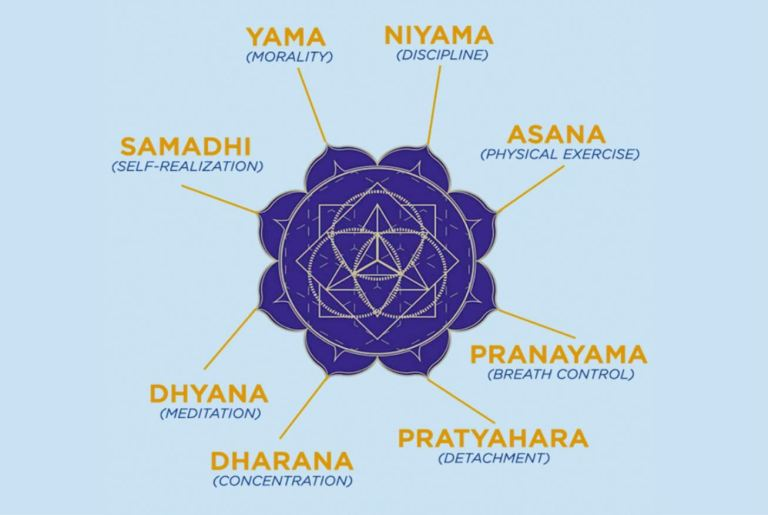
\includegraphics[width=0.6\linewidth,keepaspectratio]{images/yog22}
\end{center}

		\begin{itemize}
		\item Steps progression isn’t meant to be rigid. 
		\item For example, someone might begin the practice of an asana before they have mastered Niyama, still, they must follow the overall elements of the 8 limbs to have a wholesome growth.
		\end{itemize}
		
\end{frame}

